% !TeX root = ../projeto.tex
\newpage
%\thispagestyle{empty}
%\pagenumbering{arabic}

\section{REFERENCIAL TEÓRICO}
\label{sec:referencial-teórico}
Os serviços de diretório desempenham um papel crucial na gestão de identidades e no controle de acesso em ambientes de rede. Estes serviços são projetados para armazenar, organizar e recuperar informações sobre usuários, grupos, recursos e outras entidades em uma rede. Eles fornecem uma estrutura hierárquica que permite o acesso e a busca eficientes dos dados, seguindo o modelo de árvore, onde cada nó representa uma entrada ou objeto.

Atualmente, existem várias soluções de diretório disponíveis, cada uma com características e funcionalidades distintas. Nesta seção, será demonstrado o estado da arte atual desses serviços, com foco no Lightweight Directory Access Protocol (LDAP), que se baseia no padrão X.500, um protocolo pesado, que opera sobre a pilha completa de protocolos OSI e requer uma quantidade significativa de recursos computacionais. O LDAP é projetado para operar sobre TCP/IP e fornece a maioria das funcionalidades do X.500 com um custo muito menor, pois não precisa rodar na pilha de sete camadas OSI \cite{machado2020}.

\begin{figure}[h]
    \centering
	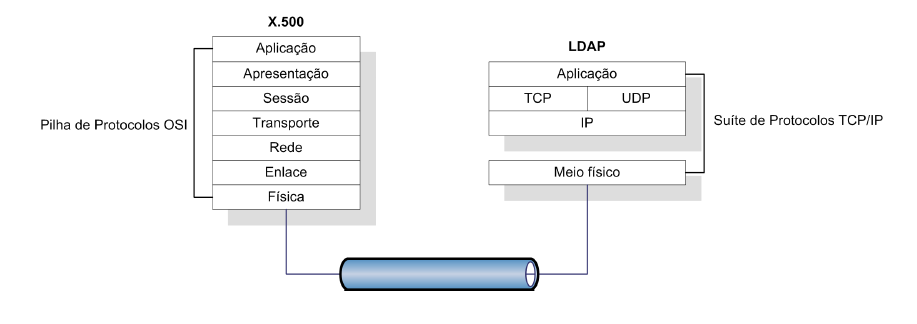
\includegraphics[scale=0.6]{projeto/textuais/CamadasX.500LDAP.png}
	\caption[X.500 sobre OSI vs. LDAP sobre TCP/IP-]{X.500 sobre OSI vs. LDAP sobre TCP/IP \cite{machado2020}.
	\label{fig:camadaX.500Ldap}}
\end{figure}

\subsection{LIGHTWEIGHT DIRECTORY ACCESS PROTOCOL (LDAP)}

Como foi citado anteriormente, o modelo de árvore de nós é usado para representar a estrutura hierárquica de um serviço de diretório LDAP. Nesse modelo, os nós são os elementos fundamentais que compõem o diretório e organizam as informações armazenadas nele.

O LDAP foi desenvolvido para ser servidor de diretório com propósito
geral, ou seja, foi desenvolvido para que os administradores possam
definir que tipo de informação vai ser armazenada pelo servidor, com clareza e
cuidado \cite{lima2021estudo}. Logo, seus nós podem representar diferentes tipos de objetos ou entidades, como usuários, grupos, computadores, organizações, unidades organizacionais, entre outros, dependendo da finalidade e do escopo do diretório.

\begin{figure}[h]
    \centering
	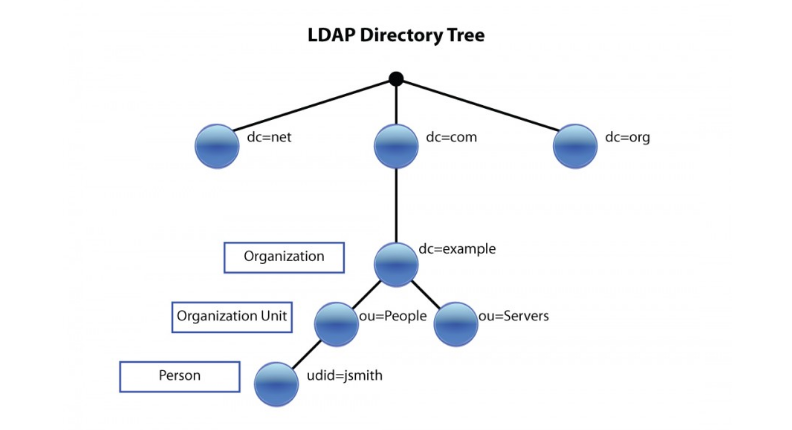
\includegraphics[scale=0.7]{projeto/textuais/LDAPTree.png}
	\caption[Exemplo da estrutura de um diretório LDAP]{Exemplo da estrutura de um diretório LDAP}.
	\label{fig:ldaptree}
\end{figure}

A organização dos dados é feita em forma de uma árvore hierárquica. Cada nó possui um identificador único chamado de "Distinguished Name" (DN). Como exemplificado na figura \ref{fig:ldaptree}, temos então os respectivos nós:
\begin{itemize}
	\item Nó raiz (Root): Esse é o ponto de partida da árvore de diretório LDAP. É o nível mais alto da hierarquia e serve como base para toda a estrutura do diretório. Pode ser imaginado como a raiz de uma árvore, de onde se ramificam os demais nós. Pode ser representado por: \textit{DN: dc=iftm,dc=edu,dc=br}.
    \item Organização (Organization): Representa uma entidade ou empresa dentro do diretório. Pode ser comparada a uma unidade dentro da própria organização ou à própria organização. Como por exemplo: "IFTM Campus Ituiutaba". É um nível abaixo do nó raiz. Pode ser representado por: \textit{DN: o=iftmitba,dc=iftm,dc=edu,dc=br}.
    \item Unidades Organizacionais (Organizational Units): São subníveis dentro da organização. Elas ajudam a organizar os dados em grupos lógicos. Cada unidade organizacional pode corresponder a um departamento ou uma divisão específica dentro da unidade da organização. Por exemplo, "PET Computação IFTM Campus Ituiutaba", é uma unidade organizacional dentro da organização "IFTM Ituiutaba". Pode ser representado por: \textit{DN: ou=petiftm,o=iftmitba,dc=iftm,dc=edu,dc=br}
    \item Pessoa (Person): Também chamadas de "usuários", são as entidades individuais dentro do diretório. Representam pessoas ou contas associadas aos serviços da organização. Cada usuário possui um identificador exclusivo e informações adicionais, como nome, endereço de email, etc. Por exemplo, "Gabriel Barco" é um usuário dentro da unidade organizacional "PET Computação IFTM Campus Ituiutaba". Pode ser representado por: \textit{DN: uid=gabriel.barco,ou=petiftm,o=iftmitba,dc=iftm,dc=edu,dc=br}
\end{itemize}

Vale ressaltar que caso a organização provedora do sistema não veja necessidade de separar a estrutura de sua organização em mais entidades, como foi mostrado, ou que a própria entidade seja a responsável pelo sistema, seguindo o exemplo acima, o nó "Organization" pode também ser representado por: \textit{DN: o=iftm,dc=iftm,dc=com}.

O LDAP utiliza uma abordagem cliente-servidor, onde os clientes enviam solicitações ao servidor para buscar, adicionar, modificar ou remover informações no diretório. O protocolo é baseado em texto e utiliza o modelo de comunicação "pedido-resposta", no qual as solicitações são enviadas pelo cliente e então, o servidor então retorna uma resposta contendo o resultado ou erro ao solicitante. 

O  protocolo  LDAP  é  padronizado  e assim  como  protocolos  de  rede,  a estrutura  de  diretório  e  serviços  providos  por  um  servidor com ele estão  todos disponíveis em RFCs (Requests for Comments).A versão mais atual é a v.3 (versão 3), um padrão desenvolvido em 1997 na RFC 2251. A especificação original foi atualizada em 2006, e RFCs de 4510 a 4519 fornecem especificações mais claras e coesivas para o LDAP \cite{lima2021estudo}.

Outra característica importante deste protocolo, é o fato de ele não ser vinculado a um sistema operacional ou provedor de serviços específico. Permitindo que diferentes sistemas e aplicativos se comuniquem e acessem informações de diretório de maneira padronizada.

Essa natureza genérica do LDAP permite que ele seja utilizado em uma ampla variedade de casos de uso, desde autenticação e autorização de usuários até armazenamento de informações sobre recursos de rede, como endereços de email, números de telefone, informações de contato, entre outros \cite{universidade-fumec}.

Além disso, o LDAP é extensível, o que significa que novos atributos e esquemas de diretório podem ser definidos e adicionados de acordo com as necessidades específicas de uma organização. Isso oferece flexibilidade para adaptar o serviço de diretório às necessidades particulares de uma infraestrutura de TI.

Atualmente existem inúmeras soluções de diretório baseadas em LDAP disponíveis no mercado, dentre as mais populares entre elas, podemos citar: OpenLDAP, Microsoft Active Directory (AD), Novell eDirectory, Oracle Internet Directory e IBM Tivoli Directory Server. Cada uma delas possui recursos específicos e atende a diferentes necessidades de gerenciamento de diretório. A escolha da solução adequada dependerá dos requisitos e do ambiente de TI de cada organização.

Na seção a seguir será explicado mais a fundo especificamente sobre o OpenLDAP, uma implementação de código aberto do LDAP que possui recursos e funcionalidades que o tornam mais eficiente e funcional para as mais diversas estruturas de rede \cite{ninjadolinux}.

\subsection{OPENLDAP}

O OpenLDAP é uma opção popular de solução de diretórios baseada em LDAP. Ele é especialmente desenvolvido para uso em plataformas Unix, mas também é distribuído para uso no Windows. Seu desenvolvimento ocorreu paralelamente ao desenvolvimento e padronizacão do protocolo LDAP. Atualmente, o OpenLDAP é mantido por uma comunidade de código livre, que conta com a participacão de diversos desenvolvedores interessados em aprimorar o funcionamento do software \cite{oliveira2010}.

Dentre as principais características deste software podemos destacar \cite{universidade-fumec}:

\begin{itemize}
    \item Suporte a IPv4 e IPv6
    \item Autenticação (Cryrus Sasl-Kerberos V, GSSAPI, Digest-MD5)
    \item Segurança no transporte – SSL e TLS
    \item Controle de acessos (ACLs)
    \item Escolha entre bancos de dados (GDBM ou DBD)
    \item Capacidade de atender a múltiplos bancos ao mesmo tempo
    \item Alto desempenho em múltiplas chamadas
    \item Replicação de base
\end{itemize}

Além disso, OpenLDAP oferece autenticação de usuários através de sua base de dados centralizada, o que facilita o controle e a correção de problemas em caso de erros nos logins dos usuários ou nas suas permissões \cite{ninjadolinux}.

O funcionamento dele envolve a comunicação entre um cliente LDAP e um servidor LDAP. O cliente emite solicitações para realizar operações de leitura, escrita, pesquisa e exclusão de dados no servidor. Essas solicitações são baseadas em comandos como, BIND (autenticação), ADD (adição de entrada), SEARCH (pesquisa), MODIFY (modificação) e DELETE (exclusão).

O pacote do OpenLDAP é composto por quatro componentes principais \cite{lima2021estudo}:

\begin{itemize}
    \item Servidores: Fornecem os serviços LDAP
    \item Clientes: Manipulam os dados LDAP
    \item Utilitários: Servidores LDAP de suporte
    \item Bibliotecas: Fornecem interfaces de programação para o LDAP
\end{itemize}

O funcionamento da comunicação desses componentes pode ser ilustrado conforme descrito na figura \ref{fig:compLDAP}:

\begin{figure}[h]
    \centering
	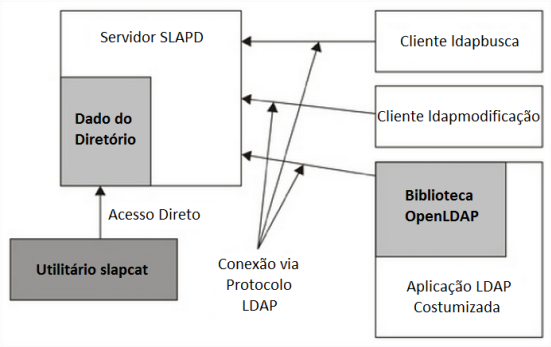
\includegraphics[scale=0.9]{projeto/textuais/ComunicacaoLDAP.png}
	\caption[Exemplo da comunicação dos componentes do OpenLDAP]{Exemplo da comunicação dos componentes do OpenLDAP \cite{lima2021estudo}}.
	\label{fig:compLDAP}
\end{figure}

No OpenLDAP o servidor principal é chamado de SLAPD (Stand-Alone LDAP Daemon), que é responsável por receber solicitações LDAP dos clientes, processá-las e fornecer as respostas correspondentes. O SLAPD funciona como um serviço em segundo plano, executando continuamente e aguardando conexões de clientes LDAP. Quando uma solicitação é recebida, o SLAPD a analisa e a encaminha para o processamento adequado. 

Este servidor tem como função armazenar dados no diretório local ou prover acesso a fontes de dados externas. Tipicamente, além de oferecer serviços de autenticação e busca de informações em diretórios, também oferece suporte nas operações de adição, exclusão e modificação de dados em diretórios. Não menos importante, esse servidor é o responsável por oferecer controle de acesso detalhado ao diretório \cite{universidade-fumec}.

Os clientes LDAP geralmente se conectam a um servidor SLAPD usando o protocolo LDAP por meio da rede, enviando solicitações para executar várias operações. Como esse protocolo opera na pilha TCP/IP, o cliente normalmente inicia estabelecendo uma conexão com o servidor de diretório. Após estabelecer a conexão, o cliente se autentica e, em seguida, executa as operações desejadas, como pesquisas, adições, modificações, exclusões e outras.

Como ilustrado na figura \ref{fig:compLDAP}, ao contrário dos clientes, os utilitários não realizam operações usando o protocolo LDAP. Os dados são manipulados em camadas mais baixas e sem mediação pelo servidor, são usados na realidade para a manutenção do servidor \cite{lima2021estudo}.

Por fim, as bibliotecas do OpenLDAP são componentes essenciais que fornecem funcionalidades para o desenvolvimento e a interação com o serviço de diretório. Elas são responsáveis por encapsular a complexidade do protocolo LDAP e fornecer uma interface de programação que facilita a criação de aplicativos que interagem com o servidor SLAPD.

Dentre as principais bibliotecas do OpenLDAP podemos destacar
\cite{universidade-fumec}:

\begin{itemize}
    \item JLDAP: biblioteca escrita em Java projetada para fornecer acesso a
    serviço de diretórios LDAP. Define duas interfaces síncronas e assíncronas
    para o LDAP de forma a atender uma ampla variedade de aplicações.
    \item JDBCLDAP: biblioteca escrita em Java que tem como função prover
    acesso a serviço de diretórios LDAP àqueles que preferem utilizar
    linguagem SQL19 e JDBC20.
    \item ldapc++: biblioteca escrita na linguagem C++ que tem como função
    prover acesso a serviços de diretórios LDAP a partir de programas escritos
    nessa linguagem.
\end{itemize}

No OpenLDAP existem também as listas de controles de acesso (ACLs), elas são mecanismos utilizados para controlar o acesso aos dados armazenados no diretório LDAP. Elas permitem definir políticas de segurança que determinam quais operações um determinado usuário ou grupo de usuários podem executar em relação aos registros e atributos do diretório.

As ACLs são configuradas por meio de regras definidas no arquivo de configuração do servidor SLAPD (slapd.conf ou slapd.d). Cada regra de ACL especifica uma combinação de filtros de entrada (entry) e atributos que devem ser correspondidos para que a regra seja aplicada.

Utilizando como exemplo a entrada uid=gabriel.barco, ou=petiftm, o=iftmitba, dc=iftm, dc=edu, dc=br, ilustrada pela hierarquia da figura \ref{fig:ldaptree}, uma regra nas ACLs para controlar o acesso aos valores dessa entrada teria
a seguinte sintaxe \cite{oliveira2010}:

\textbf{access to dn.exact=}\textit{“uid=gabriel.barco,ou=petiftm,o=iftmitba,dc=iftm,dc=edu,dc=br”}

\textbf{by dn.exact=}\textit{“uid=admin,ou=petiftm,o=iftmitba,dc=iftm,dc=edu,dc=br”} \textbf{write}

\textbf{by self read}

\textbf{by * none}

A conexão do OpenLDAP com outros servidores pode ser estabelecida para diversos propósitos, como autenticação centralizada, gerenciamento de usuários e controle de acesso. O OpenLDAP é uma solução de diretório LDAP genérica e flexível, o que permite sua integração com diferentes tipos de servidores.

Se conectando com o ProxMox, que será explicado na seção a seguir, é possível integrar o processo de autenticação dos usuários, permitindo que eles usem suas credenciais do diretório LDAP para acessar o servidor.

\subsection{PROXMOX}

O Proxmox é uma plataforma de virtualização de servidores de código aberto baseada no kernel do Linux. Ele combina tecnologias de virtualização de contêineres (LXC), e máquinas virtuais (KVM), para fornecer uma solução completa de virtualização para data centers e ambientes empresariais.

Hoje, o Proxmox se destaca por proporcionar um ambiente intuitivo e objetivo tendo em mente a gestão de máquinas virtuais. Na prática, basta poucos cliques para acompanhar, personalizar e dar instruções aos dispositivos conectados \cite{oliveira2022vantagens}.

O Proxmox permite a criação, gerenciamento e monitoramento de máquinas virtuais e contêineres em um ambiente centralizado. Ele oferece recursos avançados, como alta disponibilidade, migração ao vivo, balanceamento de carga e armazenamento compartilhado, tornando-o adequado para ambientes de produção e missão crítica.

A arquitetura dele é baseada em um hipervisor que executa a virtualização, permitindo a alocação eficiente de recursos físicos, como CPU, memória e armazenamento, para as máquinas virtuais e contêineres. O Proxmox também fornece uma interface web intuitiva, conhecida como Proxmox VE (Virtual Environment), que facilita a administração e o monitoramento das instâncias virtuais.

\begin{figure}[h]
    \centering
	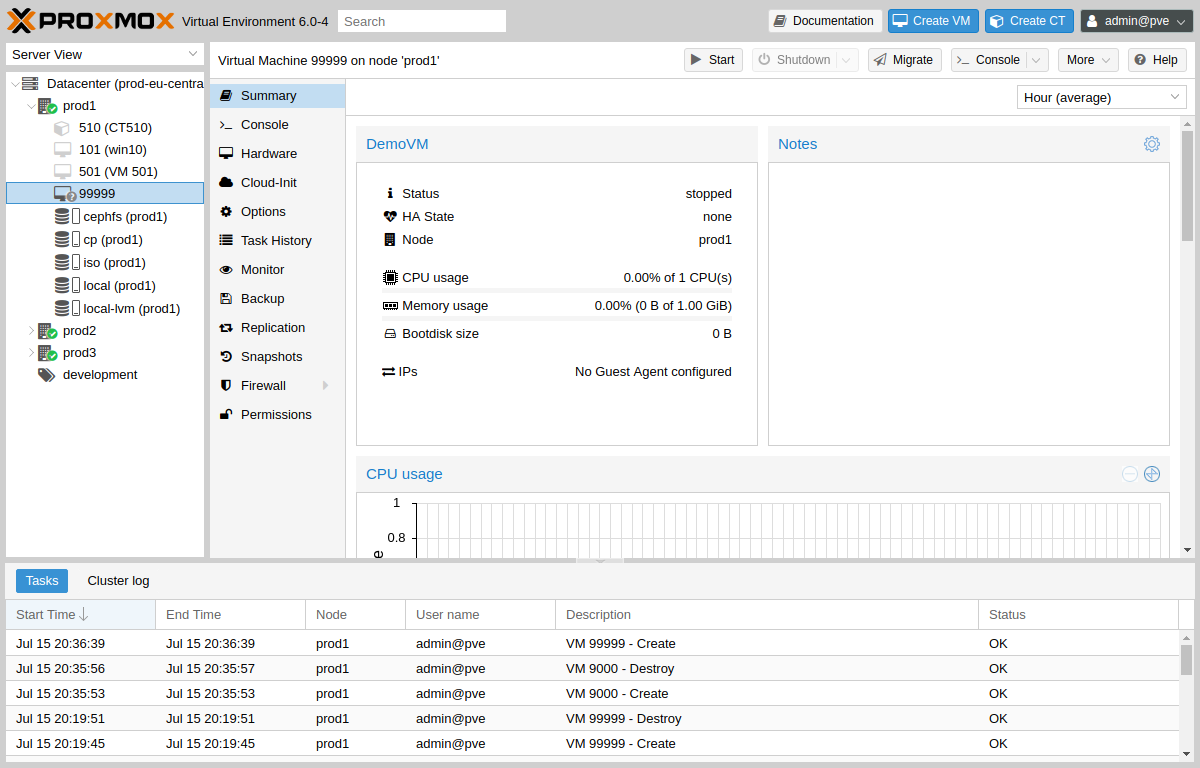
\includegraphics[scale=0.7]{projeto/textuais/gui-qemu-summary.png}
	\caption[Exemplo da interface gráfica do ProxMox]{Exemplo da interface gráfica do ProxMox. Disponível em: \url{https://pve.proxmox.com/wiki/Graphical\_User\_Interface}}.
	\label{fig:interfaceProxMox}
\end{figure}

A plataforma Proxmox é escalável e flexível, permitindo que os administradores de sistema criem e gerenciem facilmente várias máquinas virtuais e contêineres em um único local. Além disso, o Proxmox suporta recursos avançados de rede, como VLANs e balanceamento de carga, para oferecer maior flexibilidade e desempenho.

A integração do Proxmox com o OpenLDAP oferece uma série de benefícios para o gerenciamento e a segurança de um ambiente de virtualização. Alguns desses benefícios incluem:

\begin{itemize}
    \item Centralização do gerenciamento de usuários: O OpenLDAP permite a criação de uma base de dados centralizada no servidor para o armazenamento de informações de autenticação de usuários.
    \item Autenticação única (Single Sign-On): Ao utilizar o OpenLDAP como um serviço de diretório, é possível implementar a autenticação única no ambiente Proxmox.
    \item Aumento da segurança: O uso do OpenLDAP como serviço de diretório permite uma gestão mais eficaz das políticas de segurança do servidor.
\end{itemize}